\documentclass[tikz, border=2pt]{standalone}

\usepackage{helvet}
\renewcommand{\familydefault}{\sfdefault}

\usepackage[EULERGREEK]{sansmath}
\sansmath
\usetikzlibrary{arrows.meta}

\begin{document}%

\begin{tikzpicture}[line width=2pt]
\tikzset{>={Latex[width=3mm,length=4mm]}}

% % grid
% \draw[help lines] (-5, -5) grid (13, 18);

\definecolor{gold}{RGB}{255,215,3}

\definecolor{darkblue}{RGB}{2,0,139}

\node[inner sep=0pt] (figa) at (0,0)
{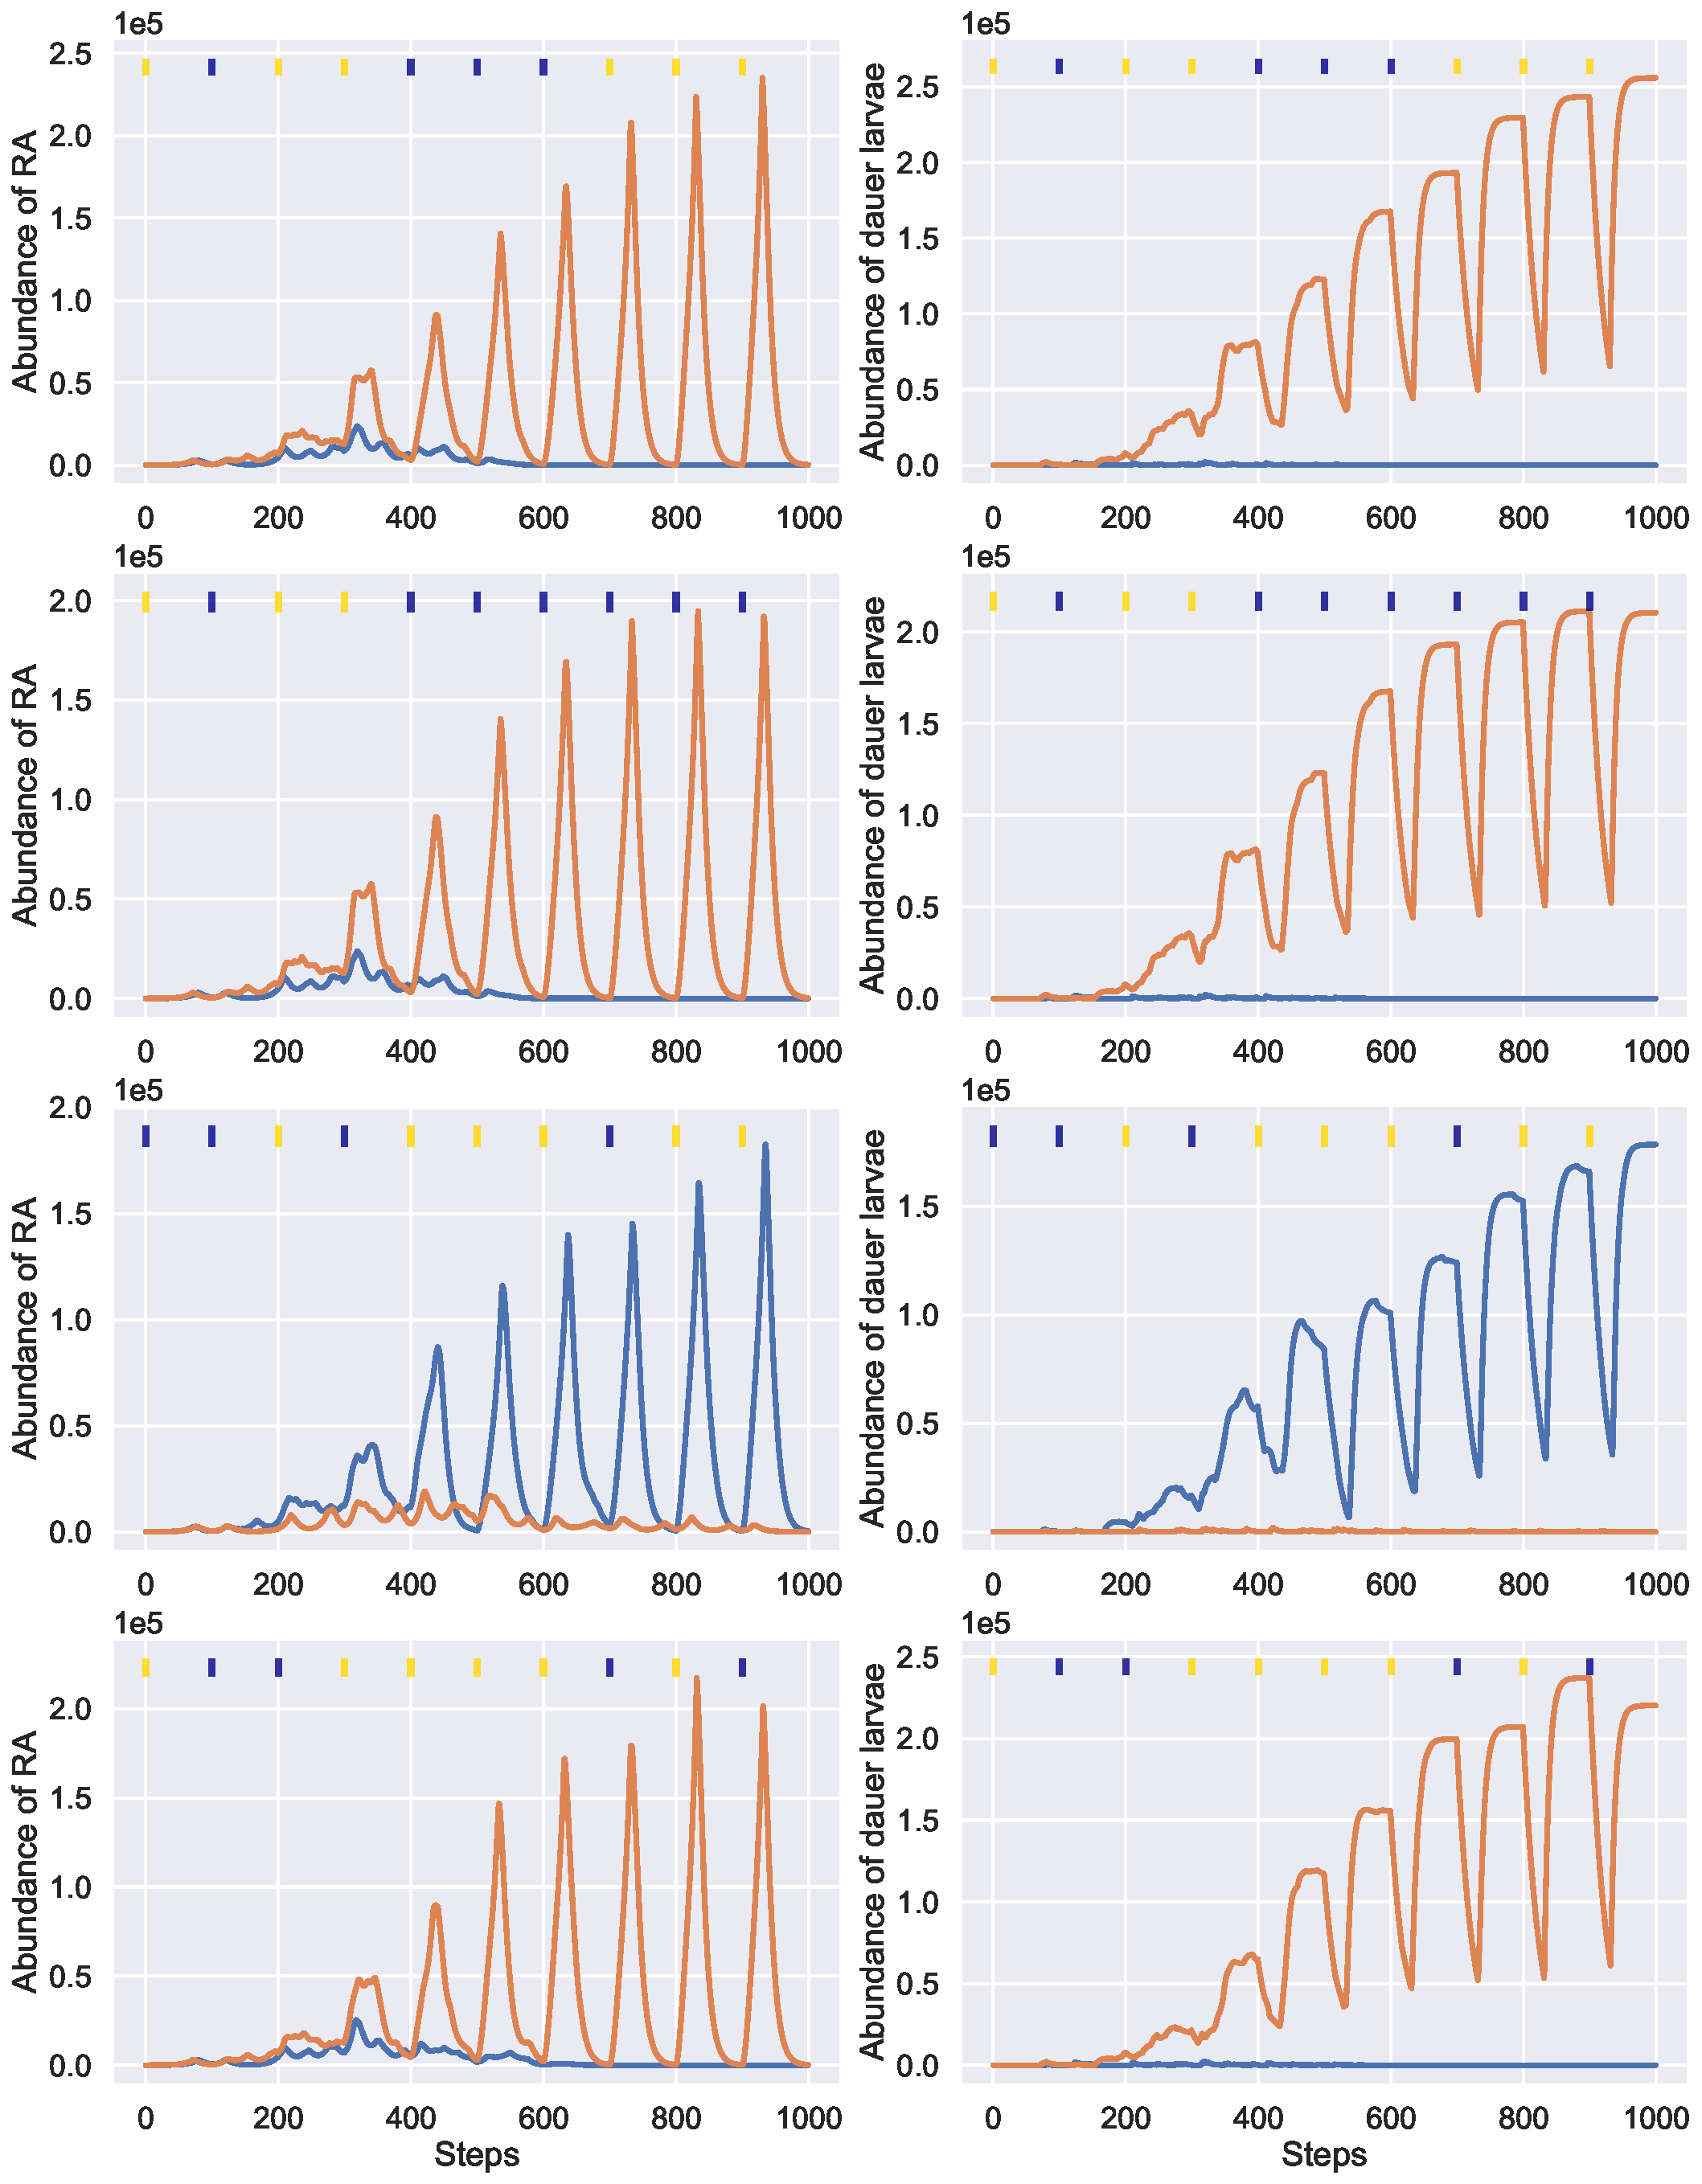
\includegraphics[width=1.\textwidth]{../meta_rand_temp_samples.pdf}};


% %labels
\draw (-6.5, 7.8) node{{\Huge\sf\textbf{a}}};

\draw (-6.5, 4) node{{\Huge\sf\textbf{b}}};

\draw (-6.5, 0) node{{\Huge\sf\textbf{c}}};

\draw (-6.5, -3.5) node{{\Huge\sf\textbf{d}}};

\node at (-3.3,8.13) [draw=none, rectangle, fill=none,rotate=0] (g1) {\sf \footnotesize Addition of \emph{E. coli} OP50};

\node at (1.3,8.1) [draw=none, rectangle, fill=none, rotate=0] (g1) {\sf \footnotesize Addition of \emph{Novosphingobium} sp. L76};

\draw [-, draw=darkblue, line width=3pt] (-5,8) -- (-5,8.3) {};

\draw [-, draw=gold, line width=3pt] (-1.2,8) -- (-1.2,8.3) {};

\draw[draw=black!20, rounded corners=5pt] (-5.2,7.8) rectangle (3.8,8.45);

\end{tikzpicture}


\end{document}